
\chapter{Mobile authoring of open educational resources for authentic learning scenarios}

%\begin{quote}
%\textbf{*Abstract:} The present paper introduces concept mapping as a structured participative conceptualisation approach to identify clusters of ideas and opinions generated by experts within the domain of mobile learning. Utilising this approach, the paper aims to contribute to a definition of key domain characteristics by identifying the main educational concepts related to mobile learning. A short literature review points out the attempts to find a clear definition for mobile learning as well as the different perspectives taken. Based on this an explorative case study was conducted, focusing on the educational problems that underpin the expectations on mobile learning. Using the concept mapping approach the study identified these educational problems and the related domain concepts. The respective results were then analysed and discussed. The core educational concepts of mobile learning identified are: �access to learning�, �contextual learning�, �orchestrating learning across contexts�, �personalisation�, and �collaboration�. The paper is original as it uses a unique conceptualisation approach to work out the educational problems that can be addressed by mobile learning and thus contributes to a domain definition based on identified issues, featured concepts, and derived challenges. In contrast to existing approaches for defining mobile learning, the present approach relies completely on the expertise of domain experts.
%\end{quote}
\vfill
The proliferation of smartphones in the last decade and the number of publications in the field of authoring systems for computer-assisted learning depict a scenario that needs to be explored in order to facilitate the scaffolding of learning activities across contexts. Learning resources are traditionally designed in desktop-based authoring systems where the context is mostly restricted to the learning objective, capturing relevant case characteristics, or virtual situation models. Mobile authoring tools enable learners and teachers to foster universal access to educational resources not only providing channels to share, remix or re-contextualize these, but also capturing the context in-situ and in-time. As a further matter, authoring educational resources in a mobile context is an authentic experience where authors can link learning with their own daily life activities and reflections. The contribution of this manuscript is fourfold: first, the main barriers for ubiquitous and mobile authoring of educational resources are identified; second, recent research on mobile authoring tools is reviewed, and 10 key shortcomings of current approaches are identified; third, the design of a mobile environment to author educational resources (\em MAT for ARLearn \em) is presented, and the results of an evaluation of usability and hedonic quality are presented; fourth, conclusions and a research agenda for mobile authoring are discussed.
\vspace{3em}

This chapter is published as: 
Tabuenca, B., Kalz, M., Ternier, S., \& Specht, M. (2014). Mobile authoring of open educational resources for authentic learning scenarios. \em Universal Access in the Information Society, \em (Special Issue: The Use of Mobile Technology and Ubiquitous Computing for Universal Access in Online Education), 1�15. doi:10.1007/s10209-014-0391-y

\clearpage

\section{Introduction}
\label{sect:1}
Situated learning  \cite{Brown1989} stress the importance of knowledge and skill acquisition in the same context in which they need to be performed; leading also to the concept of communities of practice \cite{Lave1991}. While some educational media simulate real world environments with 3D-visualizations or micro-worlds several authors have stressed the difference between a simulated environment and authentic experiences in the real world \cite{Hummel1993}, \cite{Tripp1993}. Rule \cite{Rule2006} clusters authentic learning into four themes: (1) real-world problems that engage learners in the work of professionals; (2) inquiry activities that practice thinking skills and metacognition; (3) discourse among a community of learners and (4) student empowerment through choice. The seminal article from Herrington \& Oliver \cite{Herrington2000} identifies a number of design guidelines for situated learning activities like the need to provide authentic tasks and problems as also to support the change of perspectives. 

With the availability of mobile technologies new potentials for the design and creation of authentic and situated learning materials have emerged \cite{Duval2009}. Lombardi and Oblinger \cite{Lombardi2007} identify mobile devices as one of the key technologies to support authentic learning with information access and data collection during field-based investigations. On the one hand learning support with mobile devices has aimed to increased universal access to advanced learning opportunities on the other hand the creation of learning materials in context and the documentation of authentic learning experiences have been researched. Nevertheless there are still many restrictions for the authoring support of authentic learning resources on different aggregation levels. Several research projects have demonstrated the potential of using mobile and ubiquitous devices to capture contextual information \cite{Zimmermann2005d} and recording real-life experiences \cite{Barreau2007}, \cite{Hodges2006} but this potential has remained underexploited for the process of mobile authoring of learning resources.

Within this article we refer to ''Mobile Authoring'' as the process of content creation on different levels of aggregation by using mobile technologies. Kinshuk \& Jesse \cite{Kinshuk2013} discuss the relevance of mobile authoring when capturing learning where and when it occurs. Additionally, they stress the lack of learner generated content in reusable learning objects authored for e-learning, especially with timely, relevant, and location aware examples. 
This manuscript reports about an analysis of existing mobile authoring solutions and the development and evaluation of a new mobile authoring tool  for open educational resources. In the next section we report about related work and discuss shortcomings of current mobile authoring tools. In section 3 we introduce the Mobile Authoring Tool for ARLearn (\em MAT for ARLearn \em) that we have build aiming at authentic learning environments and the related authoring activities as also the shortcomings of analyzed tools. In section 4 we introduce an evaluation of usability and hedonic quality of the \em MAT for ARLearn \em. Section 5 discusses these results and limitations of the work. Last but not least we discuss future research.

\section{Motivation and related work}
\label{sect:2}
Authoring learning resources is currently still a process that is generally conducted in front of a desktop computer making it hard to capture real-life experiences related to the actual learning situation. Most of the current authoring environments are desktop solutions that enable the deployment of the authored learning materials to mobile devices \cite{Perez-Sanagustin2012a}, \cite{Gruntjens2013}, \cite{Sampson2012}, \cite{Gicquel2011}, \cite{Mathews2010}, \cite{MartIn2009}, \cite{Cabada2009}, \cite{Kim2013}. In this scenario, the user authors an educational resource surrounded by blank walls and situated in front of a computer screen. Authoring educational resources in a mobile context is a more authentic activity that provides access to real-life experiences, which are otherwise not easy to capture. For instance, when creating a learning resource about the architectural design of a building in the physical environment and context in which the building is located, the created learning materials and documentation are expected to be very different from the materials designed on a desktop computer. The creation in-situ and perception of relevant affordances and details is expected to impact the design of instructional materials as also the learning resource selection. 

Remix and re-contexualization are key practices within the field of Open Educational Resources (OER). The combination of authentic learning scenarios and mobile authoring facilitates the connection between real-world locations and digital learning resources. Therefore the reuse and re-contextualization potential can be even larger than in traditional technology-enhanced learning scenarios. Nevertheless, different authors are skeptical on the assimilation and progress of remixing and re-contextualization practices from educators� side. Amiel \cite{Amiel2013} concludes that remixing learning resources is still not mainstream in education. Collis and Strikjer \cite{Collis2003} report little success with bringing instructors close to an actual authoring process: ''instructors do not have the time, interest, or skills''. The proliferation of smartphones and the familiarization of new generations with mobile technology are bringing students and educators closer to an authentic and contextualized authoring process and to support reuse and remix of earlier developed resources. 

The work from Mugwanya and Marsden \cite{Mugwanya2010} reviews mobile learning content authoring tools from 2002 to 2009. The authors categorize these tools according to technology used, pedagogy and usability dimensions. They summarize that the majority of the tools are developed with the goal of being integrated into Learning Management Systems (desktop computer) and stress the need to develop mobile authoring tools that empower users to author content for use in mobile environments. More recently, several authors \cite{Perez-Sanagustin2012a}, \cite{Gruntjens2013}, \cite{Sampson2012}, \cite{Gicquel2011}, \cite{Mathews2010}, \cite{MartIn2009}, \cite{Cabada2009}, \cite{Kim2013} have proposed solutions for desktop-based authoring of mobile content. These studies report about functionalities like the preparation of routes in maps, the binding of content to QR codes, or language learning content created on mobile devices to be later deployed for mobile learning support. Nevertheless these learning contents are mostly authored in front of a computer screen outside of the real context in which the mobile learning intervention is conducted later.

In contrast to desktop-based authoring, we have conducted a review of existing tools that support the mobile authoring of learning resources. There are different models classifying learning resources according to their granularity \cite{Wagner2002}, \cite{Duval2003a}. In the following, we will review mobile authoring tools aiming to shed light both on the granularity of mobile generated learning contents, and, what features do mobile authoring tools provide to foster universal access to existing learning resources. 

\subsection{Review in mobile authoring tools}
\label{sect:2_1}
The underlying search was conducted utilizing the online research repositories of the Association for Computing Machinery (ACM), the publisher Springer, Google Scholar, as well as the IEEE Computer Society. The focus on these repositories is reasonable as they cover a sufficiently large number of relevant publications. Within the ACM digital library an advanced search was performed in late January 2014 querying all articles of type journal, proceeding, or transaction that had been published since 2005 when mobile phones became more popular, and matching the keywords ''authoring AND mobile'' as part of the title. The query revealed 8 results whereof 4 were appropriate. As this query did not report enough results, a second search in the full-text matching the keywords ''authoring AND mobile AND learning'' was performed. The query revealed 1051 results where the first 30 occurrences ordered by relevance were selected. These 34 items were filtered by title and/or abstract. The rest of the repositories where analyzed analogously as illustrated in figure \ref{fig:1} The 24 resulting articles were fully analyzed and desktop-based authoring tools were discarded. This review has resulted in eight authentic mobile authoring environments listed in the appendix 1 ''Authoring tools in mobile context''.
\begin{figure}
	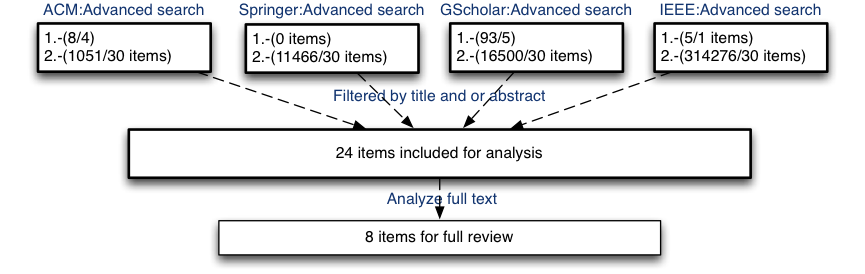
\includegraphics[width=1\linewidth]{img/fig1}
	\caption{Mobile authoring tools review procedure}
	\label{fig:1} 
\end{figure}
For a more in-depth analysis of the mobile authoring tools identified in the literature review we have compared the different granularity levels that they support in their authored educational resources. As a basis we have used modular content hierarchy from learning objects introduced by Duval \& Hodgins \cite{Duval2003a}. The result of this comparison is synthesized in table \ref{tbl:excel-table1}.
\begin{table}
  \caption{Modular Content Hierarchy in mobile authored OER}
  \label{tbl:excel-table1}
  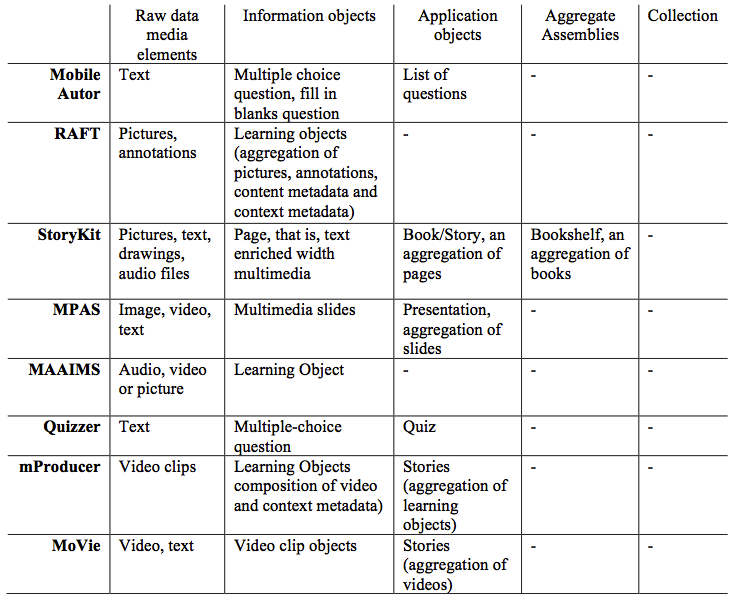
\includegraphics[width=\linewidth]{img/table1}
\end{table}
Resources that have a low granularity, such us \em raw media \em elements are highly reusable. \em Raw media \em elements include, pictures, text in the form of annotations, audios, video clips, metadata about content, metadata about standard (LOM, SCORM), or metadata about the context (GPS coordinates). \em Aggregate assemblies \em and \em collections \em have higher level of granularity but they are least reusable.

The content taxonomy presented in table \ref{tbl:excel-table1} shows that all mobile authoring tools populate two to four levels of granularity. None of the mobile authoring tools populates the level of \em collection \em in the content taxonomy. This fact indicates that so far, content authored in mobile context is not created to be part of extensive collections, but rather to be integrated in units of lower granularity. An argument for this is the lack of available tools supporting remix of learning contents. 

The analysis of these articles has resulted in the identification of 10 limitations (L1-L10) of mobile authoring tools with regard to universal access of content authored in a mobile context:
\begin{enumerate}
\item Sharing functionality. Authoring tools must feature sharing of authored educational resources in order to foster reuse and facilitate the expansion. Only one of the presented tools allows the sharing of resources created via E-Mail (\em StoryKit \em).
\item Remix support: Remixing allows authors to reuse educational resources and their rearrangement within new application contexts. Only two of the analysed tools provide support to remix resources (\em Quizzer \em and \em Mobile Author \em). While the two tools only allow remix on the \em information object \em level, remix features should be provided on different granularity levels to exploit the full potential of sharing of learning resources.
\item Recontextualization: Recontextualization is the transfer of a learning resource from one context to the other. While related concepts like repurposing \cite{Rensing2005} focus on the change of educational context, for the mobile authoring of learning resources for authentic learning scenarios the re-contextualization from one location to the other is important. The tools \em MAAIMS \em, \em Quizzer \em, \em RAFT \em and Producer support this type of re-contextualization.
\item Editing: Editing of educational resources benefits the adaptation of contents, context, and the rearrangement of the learning objects. Mobile authoring tools should provide mechanisms to support edit of educational resources. Some tools feature edit of the content (\em StoryKit \em and \em Mobile Author \em). MMAIMS feature edit of content metadata, and others feature edit of context metadata (\em Quizzer \em and \em RAFT \em).
\item Search functionality: Mobile authoring tools should provide mechanisms to support allocation of educational resources from internal or/and external repositories \cite{Tabuenca2012c}. Search of educational resources should not only be indexed on the name, description or owner of the educational resource, but also, indexed on the dimensions of the mobile context \cite{Specht2009}, namely, location, time, environment, relation and artefact identification. Hence, mobile devices can facilitate context related search of OER based on the location, time/date when the resource is useful or depending on the people or objects closer to me in a specific moment.
\item Sharing license support: Licensing is an important feature when sharing and reusing mobile content. Recent case study \cite{Amiel2013} implementing remix of OER for language learning highlights the selection of suitable licences as key consideration: ''When remixing resources a series of considerations have to take place, which are not necessarily at the forefront in a traditional process of design. First off, one needs to be sure to select resources with more open licenses.'' Hence, the license model needs to support this remixing. Creative Commons has the right tools in place to flexibly support remixing of content. None of the presented tools (See appendix 2) features any license assignment for authored content. 
\item Learning Object standard support: The implementation of Learning Object Metadata (LOM) standards facilitates content indexing and benefits the integration of OER across Learning Management Systems. Of the analysed tools three support the IMS LOM or SCORM standard: \em MAAIMS \em facilitates the creation of standardized learning objects (IMS Content Packages and standardized learning activities (IMS Learning Designs) (IMS Learning Designs; \em RAFT \em implements SCORM.
\item Availability in open app markets: Mobile authoring tools should be available in open app markets as an approach to facilitate universal access to authoring tools. \em StoryKit \em is the only mobile authoring tool available in open markets.
\item Use of sensors: Some of the apps use different sensoring functionalities to support the contextualization and improve the quality of the learning resources. \em Quizzer \em uses the compass to serve content based on the orientation. In authoring mode, \em Quizzer \em records the orientation of the user to contextualize the resource. Moreover, \em Quizzer \em supports tagging of learning resources with the user�s identifier on creation time providing some control on the ownership of the resource. Likewise, \em mProducer \em uses an accelerometer to measure the excessive amount of camera shaking recording a video, with the aim to filter blurry and unusable recordings. 
\item Interoperability. None of the tools reviewed facilitates the interoperability and exchange of educational resources among different mobile authoring tools.
\end{enumerate}

The above-presented summary shows that there is no ideal mobile authoring tool implementing all the necessary features to exploit universal access. While the availability in open app markets will be targeted at a later stage, we have taken the limitations revealed in the from the scientific literature review into the design of \em MAT for ARLearn \em.

\section{Design of the Mobile Authoring Tool for ARLearn}
\label{sect:3}
\em MAT for ARLearn \em has been designed considering the limitations enumerated in the previous section. This tool aims to provide an open environment to facilitate any user (teacher or student) to author, share, edit, remix and recontextualize educational resources to foster universal access. Hereby we describe how \em MAT for ARLearn \em was designed and which of these shortcomings are covered.

\subsection{ARLearn: Cloud-based platform for mobile serious games}
\label{sect:3_1}
The Mobile Authoring Tool has been built upon ARLearn framework, an open source platform for authoring mobile serious games, available under the GNU Lesser GPL license \cite{Ternier2012}. ARLearn is accessible for the community as a cloud based solution where authors can, without cost, create content and deploy this content to mobile devices. Approx. 450 users have used the authoring environment to create games resulting in approx. 600 active games on the platform cloud. As illustrated in table \ref{tbl:excel-table2}, learning resources in ARLearn are classified according to four different granularities in the model of content hierarchy \cite{Duval2003a}. We will further describe these objects providing some examples in the scientific literature where this platform has been used.
\begin{table}
  \caption{Granularity of learning resources in \em MAT for ARLearn \em}
  \label{tbl:excel-table2}
  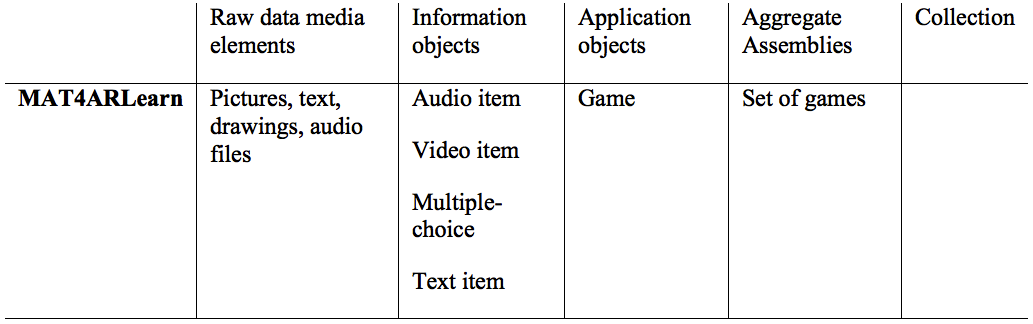
\includegraphics[width=\linewidth]{img/table2}
\end{table}
ARLearn was extended with an open repository where users can make games open, license it properly and share these with their peers. ARLearn has ben used in several authentic learning scenarios: 
\begin{itemize}
\item Recently, Schmitz et al. \cite{Schmitz2013} investigated role-playing on helping behavior with a mobile learning game to train basic life support and cardiopulmonary resuscitation. With this game they aimed at improving willingness to help in case of emergency (Figure 2).
\begin{center}
\begin{figure}[ht]
\centering
	\subfloat[Users had to allocate the defibrillator at the school and use it to save the victim.]{
		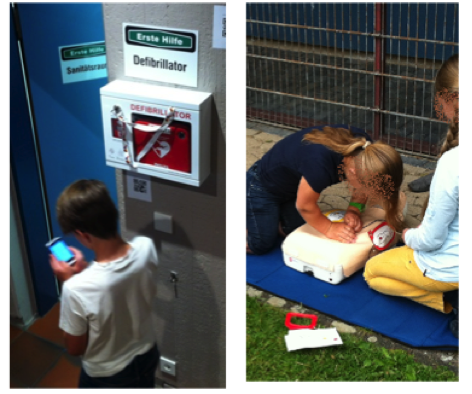
\includegraphics[width=0.5\linewidth]{img/fig2a}
		\label{fig:2a}
	}
	\subfloat[Users were instructed on the steps to follow in a cardiac arrest scenario. After the exercise, they were prompted to report the state of the victim.]{
		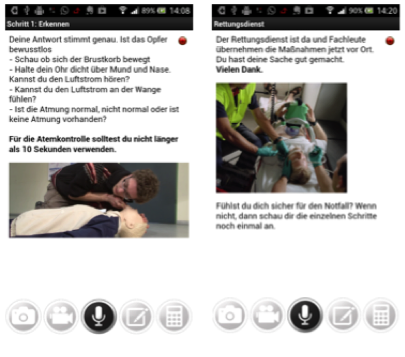
\includegraphics[width=0.5\linewidth]{img/fig2b}
		\label{fig:2b}
	}	
      \caption{Training cardiopulmonary resuscitation in schools with ARLearn \cite{Schmitz2013}.}
      \label{fig:2}
	
\end{figure}
\end{center}
\item The Mindergie games have been designed and tested at a university campus in the context of an energy conservation pilot \cite{Borner2013a}. The goal of these games is to provide incentive mechanisms to decrease the energy consumption at the workplace. Every week players were given information, tasks and challenges, e.g. a video that provides the use with hints on how to consume less electricity. 
\item In collaboration with the United Nations Refugee Agency \cite{Ternier2012z}, use cases for crisis situations were developed. These cases feature a social context through role-playing and typically zoom in on crisis situation like a hostage taking scenario. In this game employees are trained on how to react in such a situation. A game here is typically place in 5 phases: notification of the incident, assembling the team, planning, responding and negotiating. During the game players receive message according to their role. The head of office role will get a phone call from a journalist, while the staff welfare member needs to answer a call from a distressed family member.
\end{itemize}
The desktop-based\footnote{ARLearn desktop-based authoring environment. http://streetlearn.appspot.com/
} authoring environment for ARLearn (Figure 3) features the creation of games, teams, players, roles, items, and the dependencies among them. Moreover, it implements the Creative Commons (CC) licensing policy at the level of games (\em application objects \em) facilitating share and reuse across users. The games presented above are licensed under the CC attribution license. In the next section we describe the design and development of the \em MAT for ARLearn \em.
\begin{figure}
	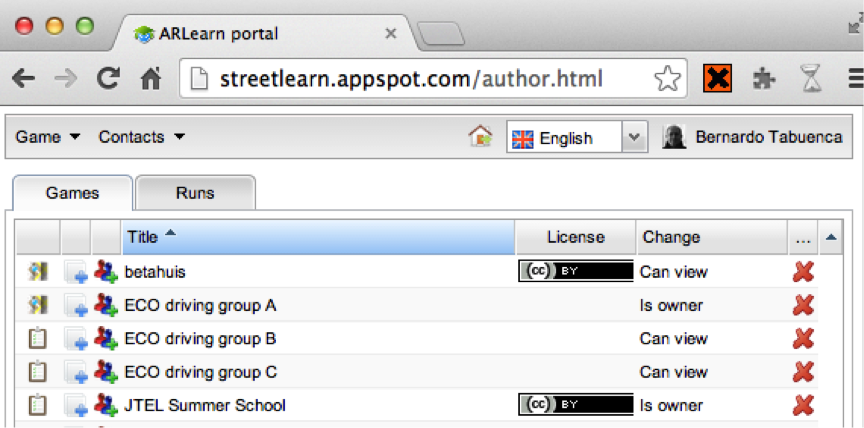
\includegraphics[width=1\linewidth]{img/fig3}
	\caption{Desktop authoring environment in ARLearn}
	\label{fig:3} 
\end{figure}

\subsection{\em MAT for ARLearn \em}
\label{sect:3_2}
The Mobile Authoring Tool complements the ARLearn desktop-based environment. Hence, a mobile game author can wander around creating items and synchronizing real world artefacts with game content. \em MAT for ARLearn \em has been designed starting a ''Mobile Authoring'' branch \footnote{\em MAT for ARLearn \em source code. https://code.google.com/p/arlearn/source/browse/?name=MobileAuthoring}  from the last release of the open source code available for the ARLearn mobile\footnote{ARLearn in Google Play. https://play.google.com/store/apps/details?id=org.celstec.arlearn2.android} client \cite{Ternier2012}. This procedure has facilitated the reuse of the already existent interfaces to access the backend via RESTful web services and the objects persisted in Google Appengine tables. The design of the tool has been performed adding functionality to the existing client following the next steps: first, we implemented the functionality to create a new game. Until now, it was only possible to create games from the desktop-authoring tool. These games are the containers of items; second, we implemented the functionality to create items so that users can create text items, video item, audio item and multiple-choice item in context recording or taking pictures with the mobile device; third, we perform the scientific literature review and identified the ten limitations for universal access; finally, these shortcomings were analysed and covered as illustrated in appendix 2.

The \em MAT for ARLearn \em features three main approaches to foster ubiquitous and universal access to educational resources: 1) an author can create and contextualize new content; 2) an existing game (or an item) can be recontextualized to a new environment; 3) licensing selection is supported to promote the reuse, revision, remixing, and, redistribution of educational materials as open educational resources (OER). 

The \em MAT for ARLearn \em features the ''My Games'' view as the starting point. Figure 4a shows the three games that the user authored for each of the architectural objects he is interested in; Figure 4b illustrates the ''Game View'' where the user can edit the resource and assign a licensing policy to share it. Clicking on the ''item tab'' (middle one) the user accesses the items that form this game. The author has the option to contextualize the content by binding it to the current coordinates, or by binding it to an existing QR code. Figure 4c illustrates the case of a user that has created a narrator item (text item) about the Church of St. Peter as an aggregation to the porticos game (\em application object \em). As he is located in an authentic environment, for example in front of the church and staring at the portico, the description inspired on the real situation is completely different from the one he would create sited on his desk and watching a picture on the screen. As the user is in a mobile context, he can also contextualize the educational resource to the current location. In this case, the user can contextualize the item with the dimension location by registering the current coordinates and radius (See top of figure 4c) clicking on the ''Bind to location button''. The user can also contextualize the item with the dimension artifact identifier whenever there would be a QR code next to the church. By clicking on the ''Bind to tag'' button, he would scan the code and the educational resource would be attached to that identifier. Next, he can edit the resource to indicate the CC license that should be assigned to the item.
\begin{center}
\begin{figure}[ht]
\centering
	\subfloat["My games" screen lists games created by the author]{
		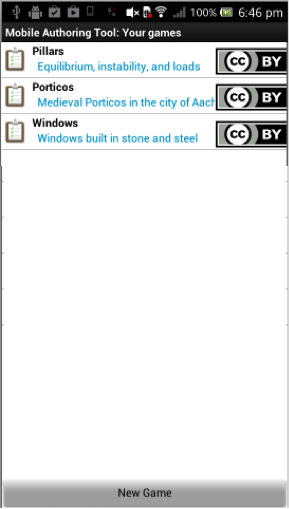
\includegraphics[width=0.3\linewidth]{img/fig4a}
		\label{fig:4a}
	}
	\subfloat[Authoring games screen]{
		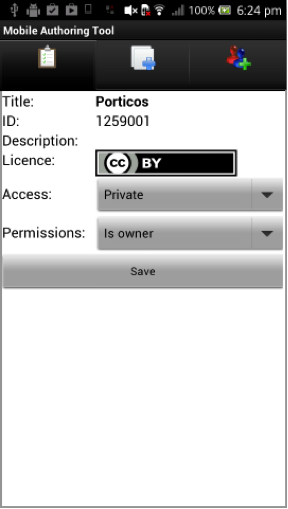
\includegraphics[width=0.3\linewidth]{img/fig4b}
		\label{fig:4b}
	}	
	\subfloat[Contextualization of educational resources]{
		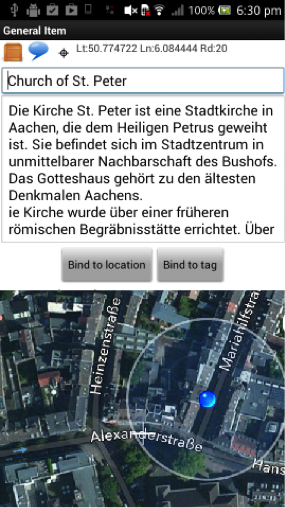
\includegraphics[width=0.3\linewidth]{img/fig4c}
		\label{fig:4c}
	}	
      \caption{Mobile Authoring Tool for ARLearn interface}
      \label{fig:4}
	
\end{figure}
\end{center}
\subsection{OER remix in mobile context}
\label{sect:3_3}
Instead of creating a new resource from scratch the user can search within the already existing OER to clone it and aggregate it without making any modification (remix), or, adapting it to the new context by updating any of the dimensions of the mobile context \cite{Specht2009} (recontextualizing). 

The \em MAT for ARLearn \em enables the user to issue a mobile OER search, to assess and to reuse an item in a new context. Users can also extend their game script by reusing a single item rather than reusing a game as a whole. Recontextualizing and remixing needs an infrastructure in place that supports flexible access to content. A search infrastructure must enable searching for content corresponding to different granularities. ARLearn supports searches from two granularities in the modular content hierarchy, namely, \em information objects \em (games), and \em application objects \em (items). Users can author games and items, and make them open access to the community. Figure 5a illustrates how licences are presented in descendent level of openness according to \cite{Vollmer2013}. Via this infrastructure, the \em MAT for ARLearn \em provides access to search functionality for items as well as for games as a whole when being in a specific context. 
\begin{center}
\begin{figure}[ht]
\centering
	\subfloat[Select level of openness for a new game]{
		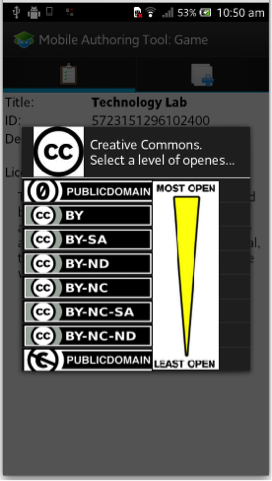
\includegraphics[width=0.3\linewidth]{img/fig5a}
		\label{fig:5a}
	}
	\subfloat[Search in already existing items for remix]{
		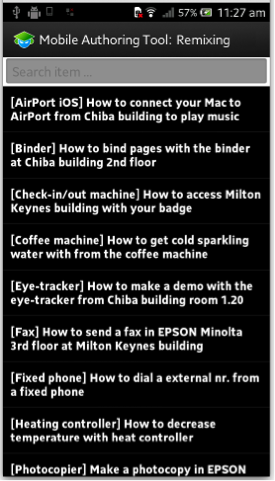
\includegraphics[width=0.3\linewidth]{img/fig5b}
		\label{fig:5b}
	}	
	\subfloat[Remix and recontextualization of a "text item" with location coordinates or artefact identifier ]{
		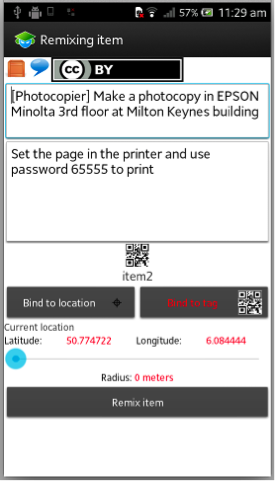
\includegraphics[width=0.3\linewidth]{img/fig5c}
		\label{fig:5c}
	}	
      \caption{Remixing and recontextualizing items with the \em MAT for ARLearn \em}
      \label{fig:5}
	
\end{figure}
\end{center}
Figures 5b and 5c illustrate a case remixing and recontextualizing educational resources in a mobile context:
\begin{itemize}
\item Remixing. The user is interested in including a video on the architecture of the Cathedral in Aachen. Instead of creating it, he uses the search tool (Figure 5b) to look for already existent educational resources. He finds an educational resource from a guided tour that somebody had previously shared. He clones the item and aggregates it as a whole into the game, without modifying it (Figure 5c).
\item Recontextualization. In this case, the user is interested in including a multiple-choice-question to assess knowledge on medieval porticos. Instead of creating it he uses the search tool (Figure 5b) to look for already existent assessments on porticos. He finds one that was previously bound to the porticos at the Cathedral of Cologne. He clones the item, modifies the context by binding it to current coordinates and radius (Figure 4c), or a QR tag (Figure 5c), and aggregates it into the game. 
\end{itemize}
The \em MAT for ARLearn \em features a new quality for recontextualization. This tool provides mechanisms to recontextualize educational resources in different dimensions like ''location'' and ''artifact identifier'' via sensors. Making content appear when the user enters a zone, is an example of binding the content to location using the GPS of the device. QR codes enable the identification of real world artifacts using the camera and the QR reader of the device. Binding content to a QR code is thus a means to synchronize them with the artifact. Image recognition, or, text recognition tags are similar approaches to recontextualize OER with the artifact identifier dimension. ARLearn allows for tagging artifacts with Radio Frequency Identification (RFID) tags or bar codes (QR, EAN-13) as an easy and open procedure to enrich physical spaces with machine-readable tags.

\subsection{OER licensing policy definition}
\label{sect:3_4}
Creative Commons fosters share and reuse. An easy to use and legally interoperable license is a critical component for the OER movement \cite{Atkins2007}. Figure 6 illustrates how OER can be legally remixed with other OER. It is important to highlight that when implementing cross-license remixing, only one third of CC�s own licenses are compatible. These combinations are illustrated in figure 6 with the smileys.
\begin{figure}
	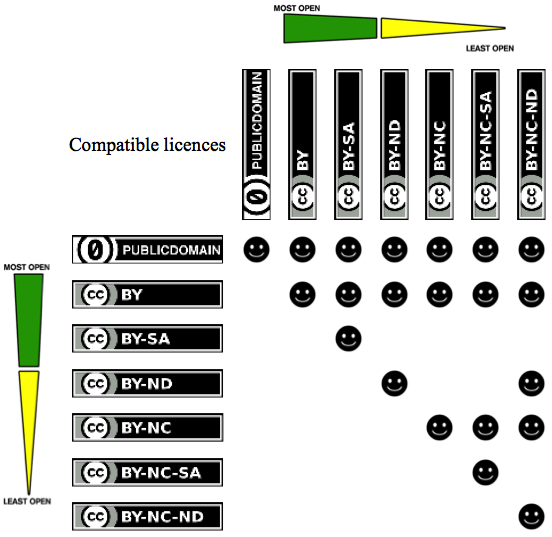
\includegraphics[width=1\linewidth]{img/fig6}
	\caption{Remix compatibility according to spectrum of freedom in Creative Commons licenses \cite{Vollmer2013}.}
	\label{fig:6} 
\end{figure}
When a game is created with open licence (different than CC-BY-NPD), all items will inherit this license by default. Nevertheless, licences from items can be consistently updated whenever both game and item licences are compatible. If a game specifies a No Derivatives (ND) licensing attribute, its items will not be searchable or reusable. In such case only the game as a whole can be reused. When a user reuses an existing game, the original author will be appropriately credited. A user that reuses a ShareAlike (SA) licensed game will not be able to restrict the access rights. Furthermore, an interesting situation occurs when a user reuses an item: if a user reuses a video that should be SA, the entire game becomes SA. 

\section{Usability Evaluation of \em MAT for ARLearn \em}
\label{sect:4}
Authoring contents with mobile technologies must be accomplished in an efficient and intuitive way that facilitates the user to create new resources in any specific context. Quantifying the usability of the Mobile Authoring Tool is key to determine how suited is the system to be used across contexts. We have conducted an evaluation of usability and hedonic quality of the \em MAT for ARLearn \em tool. In this section we present the methods, instruments and results of the evaluation.

\subsection{Method and participants}
\label{sect:4_1}
This study was conducted in February 2014 at the Open University of The Netherlands. An invitation was distributed via E-Mail with the aim to recruit participants for an experiment within the Technology Enhanced Learning Lab. Seven employees (AVG age = 34, male, all smartphone owers) voluntarily reacted to the invitation. The experiment was performed during one day with a time limitation of 30 minutes per participant and the participation was not rewarded.

In the instruction phase the participants were introduced the concept of ''mobile authoring'' as the process of producing content by building up materials in the authentic context where these artifacts or persons are normally interacting, in order to build learning ecologies. They were prompted to create a welcome game for new employees at the lab that should describe relevant resources at the workplace like technological equipment (scanner, heating control, fax, photocopier, WI-FI, coffee machine, etc.), people (room-mates, project colleague, etc.), and descriptions on how to get acquainted with the work at the institute. We suggested producing resources with a specific purpose so they can be further reused by forthcoming participants (e.g. a new employee, labour risks at your workplace, measures for energy saving at workplace, etc.). 

As illustrated in figure 7, the mobile authoring phase comprised the creation of one text item, one video item, one audio item, and one multiple-choice question that people could use to collect the assessments for these artifacts (e.g. quality of the printer, strength of the WI-FI signal in specific meeting rooms), and remix one item by choosing it from the list of shared items and edit it for reuse. Participants are asked to contextualize items by binding them to tagged artifacts (QR codes) or coordinates (GPS location). Likewise, participants were able to recontextualize items by remixing already tagged artifacts and editing the information of the context. In the last phase, participants were prompted to fill in a usability questionnaire and provide qualitative input about the hedonic quality of the tool.
\begin{figure}
	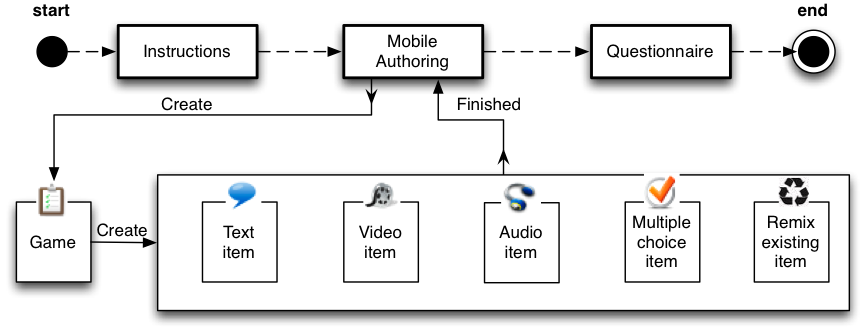
\includegraphics[width=1\linewidth]{img/fig7}
	\caption{Flow of the experiment. UML-State diagram}
	\label{fig:7} 
\end{figure}

\subsection{Instruments}
\label{sect:4_2}
The material for the study consisted in a first introduction of the experiment with a set of instructions to be read on paper, an Android smartphone (Sony XPeria S) with the \em MAT for ARLearn \em installed in it, and a desktop computer for accessing the questionnaire and the Reactiondeck toolkit. \em MAT for ARLearn \em requires an Internet connection to synchronize resources with the ARLearn backend.

The System Usability Scale (SUS) was used for the evaluation of the usability \cite{Brooke1996}. The SUS scale consists of 10 questions with a five-point Likert scale, where item directions are changed in each question. The results of the survey were recorded in an online questionnaire. Based on the current literature, a SUS score above 68 (SD:12,5) is rated as usability score above average. This analysis have followed the recommendations from Sauro \cite{Sauro2011} so that the results can be mapped and benchmarked against 446 previous studies and 5000 individual responses.

Hassenzahl has discussed the limitations of taking only into account usability and he has proposed in addition to take into account the ''hedonic quality'' \cite{Hassenzahl2001} of an interface. Hedonic quality is defined as the non-task related quality dimensions like ''accessibility'' or ''originality''. We employed the Reactiondeck toolkit developed by Benedek and Miner at Microsoft Research to assess these aspects \cite{Benedek2002}. These product reaction cards have been transferred to a digital version and published as Reactiondeck toolkit \cite{Storm2012}. Thus, participants were asked to select 6 product reaction cards that describe the emotional appeal of the mobile applications best and provide arguments on the selection (See Figure 8). After choosing the cards, users were invited to argue in an open text box why did they selected that card.
\begin{figure}
	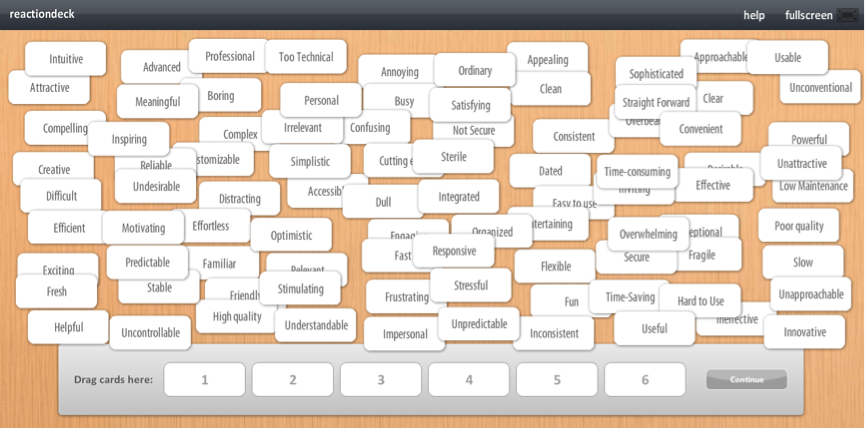
\includegraphics[width=1\linewidth]{img/fig8}
	\caption{Evaluation of hedonic quality with the Reactiondeck \cite{Storm2012}.}
	\label{fig:8} 
\end{figure}

\section{Results}
\label{sect:5}
Participants created (audio, text, video) resources to explain how to extend notebook�s screen to a bigger display, how to setup the fax, how to get cold sparkling water from the coffee machine, how to use the badge to access different buildings or how to play a demo in the eye-tracker of the lab (Figure 5b). Participants created multiple-choice questions to rate the quality of the printer, how clean is the lab, or the quality of the coffee machine. Participants remixed items like the photocopier instructions that only differed in the password depending on the building within the campus, or scanner instructions that differed in some steps depending on the brand of the device, and plugging the display that differed on the operating systems of the notebooks.

\subsection{Usability evaluation}
\label{sect:5_1}
The evaluation of the usability shows that \em MAT for ARLearn \em has a mean score of 80 (SD = 7.2), which is remarkably above average (SUS more than 68). Items 4 and 10 from the questionnaire were taken as subscale for learnability. Average learnability score was 17,81 where two participants (user 2 and 8) rated slightly below average. Items 1, 2, 3, 5, 6, 7, 8, 9 contribute to the construct usability where average score was 62,81 and only one participant rated below average (user 3).
\begin{figure}
	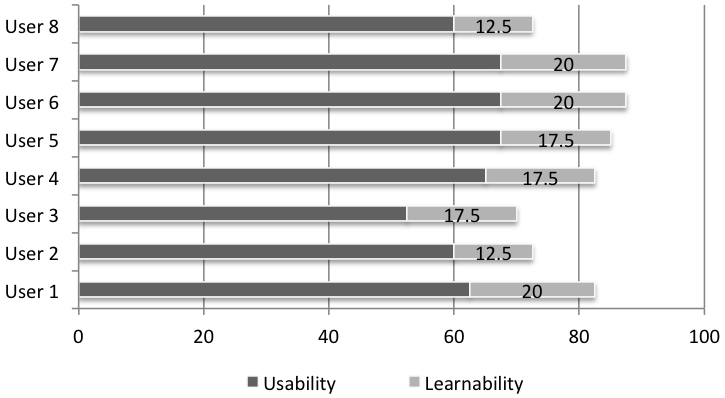
\includegraphics[width=1\linewidth]{img/fig9}
	\caption{Evaluation of Usability and Learnability with the System Usability Scale (SUS) \cite{Brooke1996}.}
	\label{fig:9} 
\end{figure}

\subsection{Hedonic quality evaluation}
\label{sect:5_2}
The Hedonic quality evaluation harvests adjectives that define the interface and usability of the tool considered in terms of pleasant (or unpleasant) sensations. Figure 10 illustrates which were the most selected adjectives to determine the hedonic quality of the \em MAT for ARLearn \em. ''Organized'' and ''Usable'' were the most voted adjectives by the participants (n=4). E.g. regarding the organization users argued: ''The distribution of items, icons and buttons within the screen is consistent'', ''The interface is clear, and there are not useless elements on the screen. All of them are self-explanatory''. These adjectives highlight a suitable distribution not only of the functionality across screens, but also of the elements (buttons, images, text boxes, etc.) used within the screens. Regarding the ''usability'' participants argued: ''The tool is intuitive and I feel confortable using it'', ''All choices for authoring are self-explained thus the tool is easy to use''. Three participants selected ''Easy-to-use'' and two participants selected ''accessibility'' arguing ''It is easy to get access to configuration procedures of artefacts through mobile devices''. These adjectives reveal an appropriate usability of the tool since participants could intuitively navigate without instruction and based on what they felt to be necessary. 

One participant highlighted the importance of providing open access to authored resources ''It is nice to share knowledge with others''. This comment recognises the benefits of openly sharing knowledge as a way of actively promoting innovation, developing educational capacity and speeding up the processes by which researchers and academics review and build on each other�s work. On the other hand, the willingness of users to share their identify tagging authored educational resources with a suitable licence keeps being a controversy. In fact, two-participants reported their reluctance selecting the card for ''not-secure'' and arguing that ''The identity of the user might be in danger when sharing resources'', ''I am not happy sharing my identity when sharing content''. 
\begin{figure}
	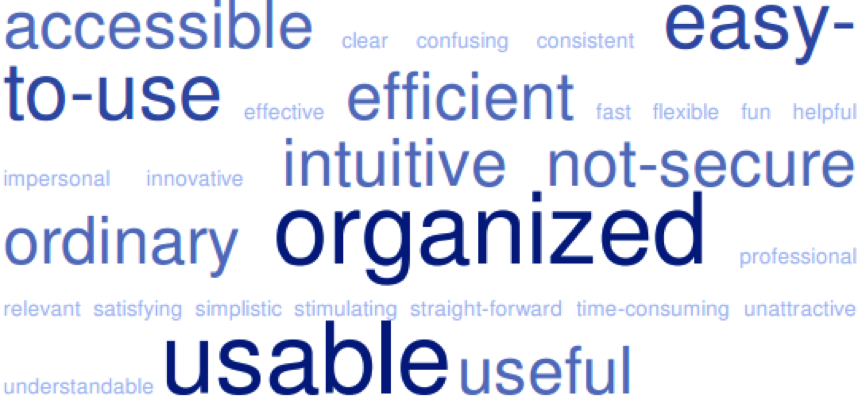
\includegraphics[width=1\linewidth]{img/fig10}
	\caption{Tag cloud visualization for the measure of hedonic quality.}
	\label{fig:10} 
\end{figure}

\section{Discussion and Conclusions}
\label{sect:6}
The article has introduced the lack of authenticity in situated learning scenarios of desktop-based authoring systems in contrast to mobile-based authoring systems where resources can be enriched with users� context \cite{Specht2009}, \em namely \em , \em  location \em, \em time \em, \em environment \em, \em relation \em and \em artefact identification \em. This manuscript proposes the use of mobile authoring tools not only as a solution to cover this gap, but also to foster universal access to educational resources. The review of scientific literature has revealed eight mobile tools for authoring of educational resources in a mobile context. These resources have been classified according to the Modular Content Hierarchy model \cite{Duval2003a}  (table \ref{tbl:excel-table1}) with the aim to identify the grain of their authored resources towards the definition and the levels they can aggregate. Based on an analysis of these tools we have recognized ten shortcomings (L1 to L10) mobile authoring tools should cope to foster universal access to educational resources authored in a mobile context (see appendix 2). 

These features have influenced the design and development of the \em MAT for ARLearn \em tool. In contrast to the existing standalone tools reviewed in this manuscript, \em MAT for ARLearn \em has a scripting environment for mobile serious games for learning in the background. \em MAT for ARLearn \em has extended the state-of-art of authoring tools featuring 7 of the 10 limitations concluded in the literature review, namely,  (L1) share, (L2) remix, (L3) recontext, (L4) edit, (L5) search, (L6) licence support, (L9) use of sensors. This tool features searching, editing and sharing of learning OERs via Creative Commons licences facilitating the remix of contents. Moreover, \em MAT for ARLearn \em features the creation and contextualization of educational resources on two of the dimensions of the mobile context \cite{Specht2009}:
\begin{itemize}
\item Location. Users can bind authored resources to locations. E.g. an audio recording on a specific architecture linked to the geographical coordinates (longitude, latitude, radius) of a church (Figure 4c). Location coordinates can be obtained via GPS sensors in mobile phones.
\item Artefact identity. Users can bind authored resources to tags attached to physical objects. E.g. text instructions on how to use a photocopier linked to a QR code (Figure 5c). Barcodes or NFC tags are instances of artefact identifiers accessible via sensors in mobile devices.
\end{itemize}
Results of a usability evaluation have confirmed that the tool has usability above average and that users understand the functionalities of the tool. These findings are reinforced by the hedonic quality evaluation conducted. We believe that mobile authoring tools that allow for content sharing under open content licensed will be a key enabler for building an ecology of digital learning resources which are freely available in the direct environment of learners and which can be re-used, adapted and recontextualized. Moreover, both the measure of �usability� and �hedonic quality� presented in this manuscript, can be taken as a reference for forthcoming developments of authoring tools serving as a base for future quantified and qualified comparisons. 

The review of authoring tools presented in this manuscript is limited to systems found in scientific literature. This research should be extended to the ones existing in open app markets (Android, iOS, Windows, Blackberry, etc.). 
\em MAT for ARLearn \em is currently in BETA version and will be released in the Google Play market as one more feature within the framework (L8). 

In future research, we will develop and evaluate further features to (re)contextualize learning contents with the pending dimensions of the mobile context \cite{Specht2009}: time (e.g. a video recording on an specific historic which is only made available to appear on anniversary dates); relation (e.g. an educational resource that is only made available to appear when all the members of a group are together); environment (e.g. ''whenever the temperature is higher than 40 degrees, play an audio item on measures to prevent dehydration'').



